\section{Methodology and Implementation}\label{sec:methodology}

This chapter describes the methodology and implementation. It begins with the construction of the TTF return series from the source data and the preparation of the options data, followed by the description of the model architecture, the training setup and the adaptations to the reference Fin-GAN implementation. Next, the experimental design and the evaluation methodology are introduced. The setup for the option pricing procedure is described, followed by the benchmark models. The chapter closes with the software environment.

\subsection{Data Pipeline}\label{sec:data-pipeline}
Two datasets are used in this thesis. The first is the TTF futures dataset, which is used to train and evaluate the model. The second is the TTF options dataset, which provides the market prices for the benchmark in Sec.~\ref{sec:pricing-setup}.

\subsubsection{Futures Data}\label{sec:futures-data}
The futures data was obtained from BASF's Bloomberg infrastructure and covers
TTF natural gas futures for the first three nearby contracts between January
2010 and April 2026. The data is distributed as three schemas: contract prices, contract metadata, and monthly listings of active contracts.

\textbf{Daily settlement prices.} This schema provides the price history of the contracts in the dataset.  Each contract is observed once per trading day, identified by contract symbol and trading date. Each record contains opening, high, low and daily closing prices in EUR/MWh, trading volume and open interest. Coverage of these fields varies considerably with how actively a contract was traded and how far from expiry it is. The closing price is the exception and is available throughout the whole dataset. Additionally, it falls outside the intraday high–low range for \num{7712} of \num{25884}  records, or \SI{29.8}{\percent}. The deviation is small in most cases, with a median of \num{0.10} EUR/MWh, but reaches up to \num{42.26} EUR/MWh. The latter confirms that it is a settlement price set by the exchange rather than a price at which trading occurred.

\textbf{Contract metadata.} This schema provides static attributes per unique contract in the dataset. The expiry date provided per record is used to rank contracts by time to maturity in Sec.~\ref{sec:m1-construction}. All contracts in the dataset are physically delivered instruments traded on ICE Endex and quoted in EUR/MWh. First and last trading dates, notice dates and delivery dates are also recorded.

\textbf{Contract listings.} This schema records which contracts were active on the market, as monthly snapshots taken on the first calendar day of each month. Each contract is observed once per snapshot. Together with the expiry dates, the listings determine which contract is the front month on a given date, as described in Sec.~\ref{sec:m1-construction}.

\subsubsection{Front-Month Series Construction}\label{sec:m1-construction}
As described in Sec.~\ref{sec:futures-data}, the contract listings and the
contract metadata each hold part of the information required to identify
the front-month contract. The listings record which contracts were active in a
given month, while the metadata records when each contract expires. Therefore, the expiry dates were joined onto the listings by contract symbol. As a result, each listing record carries the expiry date of the contract it refers to. 

The contracts were then sorted by expiry date within each monthly snapshot and the earliest-expiring one was kept. This gives the front-month contract for that month. Since the snapshots are monthly, but the series must be daily, each trading day was assigned the front-month contract from the most recent snapshot on or before that day.
The settlement price of the selected contract was then added for each trading day, matching on trading date and contract symbol. The trading days without an available settlement price were discarded. The resulting series contains \num{3998} trading days spanning 2010-01-04 to 2026-04-24, with settlement prices ranging from \num{3.509} to \num{339.196}~EUR/MWh. The construction of the front-month series is implemented in \texttt{build\_front\_month.py}.

Since the front-month contract is replaced at each expiry, the series is not the price history of a single instrument. The listings are monthly snapshots, so the front-month contract switches on the first trading day of each month. The days between the last trading day of the contract and the next listing do not carry a settlement price. These days were discarded from the series.\footnote{Trading in a TTF futures
contract ceases two UK business days before the first day of the delivery month.} Returns spanning a contract transition cover two to six calendar days, with a median of four, and reflect the change in the price level as well as the difference between the two contracts. Across the \num{195} transition days in the sample, the standard deviation of log returns is \num{0.071}, compared to \num{0.037} on all other days. When the transition days are excluded, excess kurtosis falls from \num{14.91} to \num{14.65}, and skewness from \num{0.70} to \num{0.26}.\footnote{Skewness and excess kurtosis are computed with the sample estimators $g_1$ and $g_2$ of Eq.~\eqref{eq:g1-g2}.} Transition days contribute little to the tail weight of the series, but they are responsible for most of its positive skew. 


The transition effect described above is preserved and quantified rather than removed, since restricting the analysis to a single contract would reduce the sample to a few months.

\subsubsection{Return Definition}\label{sec:return-definition}
The original Fin-GAN input series is built from two returns per day \parencite{vuleticFinGANForecastingClassifying2024}. The first is the intraday return, from the opening to the closing price and the second is the overnight return, from one closing price to the next opening
price. The return of the corresponding sector ETF is then subtracted from each entry. This isolates the part of the movement specific to the asset.

Neither step has been adopted for the TTF futures dataset. The two-return scheme requires opening and closing prices that are both traded prices. As shown in Sec.~\ref{sec:futures-data}, the daily price in this dataset is a settlement price set by the exchange. A return computed between the opening trade and the settlement price would therefore combine two different price concepts.

Additionally, the excess-return step requires a benchmark that leaves a meaningful residual when subtracted. In the case of equities, subtracting the sector ETF return removes the market-wide component and leaves the movement specific to the individual stock. European natural gas has no comparable instrument.

As a substitute, the second nearby contract was considered. However, the difference between the first and second nearby returns is a calendar spread return, as described in Sec.~\ref{sec:futures}. A model that is trained on it would learn how the gap between two contracts moves, not how the gas price itself moves. Option payoffs depend on the price level at expiry, so a model trained on spread returns could not be used to price options.

Therefore, the dataset was constructed from daily logarithmic returns of the front-month settlement price. Returns are approximately stationary and therefore comparable across the sample period. Additionally, log returns are additive across time and allow price levels to be recovered exactly from simulated returns. The latter is required for the Monte Carlo procedure
in Sec.~\ref{sec:pricing-setup}.

\begin{equation}\label{eq:logreturn}
    x_t = \log\!\left(\frac{P_t}{P_{t-1}}\right),
\end{equation}
where $P_t$ is the front-month settlement price on trading day $t$.
The transformation gives \num{3997} return observations.

\subsubsection{Data Split}\label{sec:data-split}
The return series was split chronologically into training (\SI{80}{\percent}), validation (\SI{10}{\percent}), and test (\SI{10}{\percent}) sets using the proportions of \textcite{vuleticFinGANForecastingClassifying2024}. Training covers 2010-01-05 to 2023-01-18
validation 2023-01-19 to 2024-09-04 (\num{399} returns), and test
2024-09-05 to 2026-04-24 (\num{401} returns).
\begin{figure}[htbp]
    \centering
    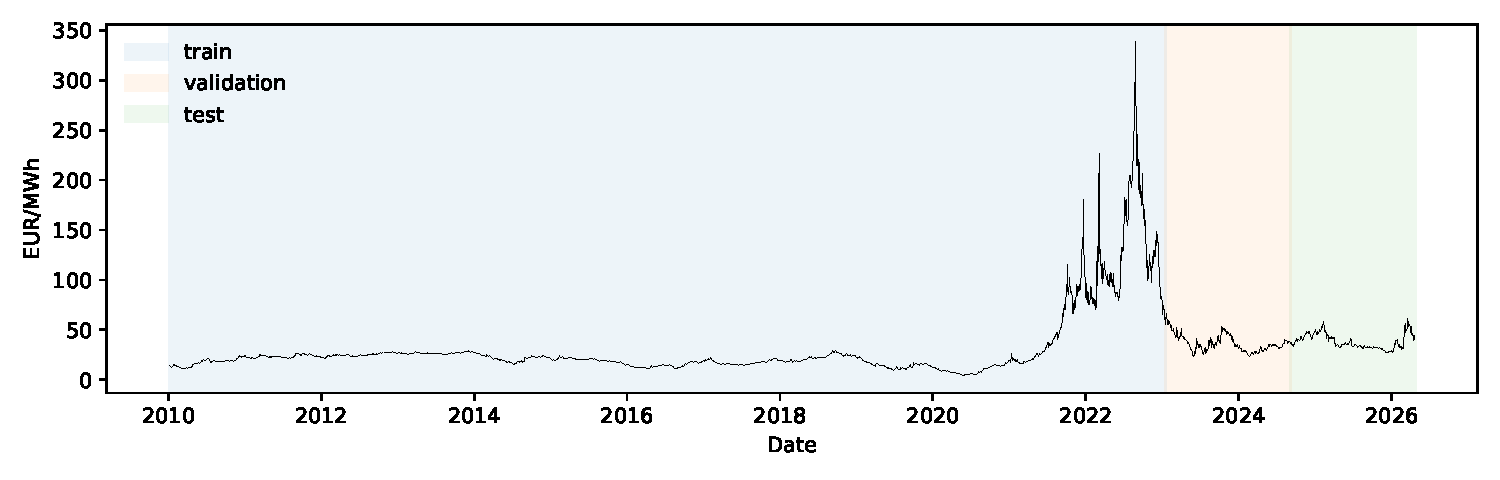
\includegraphics[width=\textwidth]{figures/ttf_price_split.pdf}
    \caption{TTF train, validation and test data split}
    \label{fig:ttf-price-split}
\end{figure}

The chronological split was explicitly used to avoid look-ahead bias. Following the current split, the 2021 to 2022 price disruption discussed in Sec.~\ref{sec:gas-markets} falls entirely within the training period, and the 2026 disruption falls entirely within the test period, as seen in Fig.~\ref{fig:ttf-price-split}.

Sliding window matrices were constructed for each split separately, so that no window spans a split boundary. The window was moved forward by one trading day.

\subsubsection{Options Data}\label{sec:options-data}

The TTF options data was obtained from Databento and covers ICE Endex TTF natural gas options. Contract records span March 2019 to June 2026, and daily settlement prices are available from March 2023 to June 2026. The price coverage contains the full test split of Sec.~\ref{sec:data-split}. The data is distributed as five schemas: Definition, Statistics, Best bid and offer (BBO), Open High Low Close Volume (OHLCV), and Status. 

\textbf{Definition.} Contract metadata is provided per instrument in the dataset. All options are European and quoted in EUR/MWh, matching the futures dataset of Sec.~\ref{sec:futures-data}. The underlying of each option is a front-month TTF futures contract. Instrument classes present in the dataset are calls, puts, calendar spread instruments and multi-leg instruments. Calendar spread instruments hold a long position in one delivery month and a short position in another. Their value depends on the calendar spread of Sec.~\ref{sec:futures} rather than on the price level. Multi-leg instruments combine multiple options into a single contract. Neither class has a strike price, so the payoff described in Sec.~\ref{sec:options} is undefined for them. Only call and put options were kept. This leaves \num{15005854} of the \num{56882528} records in the schema, split evenly between calls and puts. Strike prices range from \num{0.50} to \num{1000} EUR/MWh across \num{510} distinct values, and contracts carry \num{142} distinct expiry dates, one per calendar month. This schema is an event log, where each record describes a change in the metadata of a contract. The most recent record for each contract was retained, giving \num{35952} contracts.

\textbf{Statistics.} Daily statistics are provided per statistic, contract and trading day. The schema holds \num{99307437} records, of which \num{60664334} are put and call options. It contains settlement prices and implied volatilities, alongside further statistics that are not used, leaving \num{17424688} records. The implied volatility is published by the exchange, so the numerical procedure of Sec.~\ref{sec:implied-vol} is not required for the market prices. The dataset contains final and preliminary records, of which only the final ones are kept. \num{5807828} records are retained for settlement prices and \num{5812246} for implied volatilities. \num{392904} contract-days carry a duplicate record, of which \num{4128}, around \SI{1}{\percent}, carry a different price. These cluster on a few dates and are consistent with revisions published by the exchange. To ensure that revised prices are used, the record with the highest sequence number was retained. The resulting panel contains \num{11231588} records for \num{20252} contracts, around \SI{56}{\percent} of the \num{35952} contracts in the dataset.

\textbf{BBO.} The schema records the best bid and ask prices in a sequence of snapshots through each trading day. A bid and an ask together are referred to as a quote. The quote is two-sided when both are present. The schema covers the period from 2023-05-02 to 2026-06-26. However, two-sided quotes are almost absent at the start of that period, with \num{2485} in 2023 and \num{2069} in 2024 against \num{25969129} in 2025. The test split of Sec.~\ref{sec:data-split} begins on 2024-09-05, so the quotes would cover only part of it. 

\textbf{OHLCV.} The schema records the opening, high, low and closing prices, together with the trading volume, in one-minute bars. The schema covers 2023-03-20 to 2026-06-26. Each bar summarizes the trades in a single contract over one minute. Of the \num{365892} bars, \num{340313} are on-exchange and the remainder are off-market trades that print at different prices. Only \num{4327} of the \num{20252} contracts with settlement prices have any trades, around \SI{21}{\percent}. Out of all the days when an option received an official settlement price, only \SI{0.47}{\percent} also had a trade. As a result, the schema does not provide a continuous price series. 

\textbf{Status.} The schema records whether each contract was open for trading and whether it was open for quoting. The schema does not provide price information and is not used in this thesis.

The contract definitions and daily statistics each hold part of the information required. The definitions hold the strike price and the expiry date, while the statistics hold the settlement price and the implied volatility. The two schemas were joined by contract identifier. The front-month series of Sec.~\ref{sec:m1-construction} was then joined by the trading date to provide the front-month settlement price and the moneyness defined in Sec.~\ref{sec:options} for each option. The moneyness of an option is exact only when the underlying is the front-month contract, since the series carries the price of whichever contract is front month on that date. This holds close to expiry. Each row of the panel is one contract on one trading day, and also carries the number of days from the trading date to expiry. In total there are \num{5615794} records for \num{20252} contracts. The days between the last trading day of a contract and the next front-month listing do not carry a front-month settlement price, so \num{268598} records have no moneyness. A further \num{181950} records fall after 2026-04-24, the end of the futures series, and also do not carry moneyness. The construction of the options panel is implemented in \texttt{build\_options\_panel.py}.

The panel spans March 2023 to June 2026, while the test split of Sec.~\ref{sec:data-split} covers September 2024 to April 2026. It was restricted to the test split, resulting in \num{1763210} records for \num{9144} contracts. Three groups of records were then filtered out. \num{5062} records on the expiry date have a time to maturity of zero, so no pricing method applies to them. A further \num{81584} records fall on the days without a front-month settlement price, described above. Lastly, a moneyness band of \num{0.5} to \num{2.0} was applied. Since the median settlement price falls smoothly with moneyness, there is no natural break in the data, so the bounds were set as follows. Below the \num{0.5} lower bound, the implied volatility rises and becomes erratic. Almost all the option value is the amount it would pay if exercised immediately, and the volatility is recovered from the small remainder. Above the \num{2.0} upper bound, the median settlement price approaches the exchange minimum tick of \num{0.005}, so the price does not carry information. The resulting panel contains \num{1250980} records for \num{7208} contracts. The filtering of the options panel is implemented in \texttt{filter\_options\_panel.py}.
\subsection{Architecture, Setup and Adaptations}\label{sec:model}
The model follows Fin-GAN, with the architecture and training setup taken from the reference implementation of
\textcite{vuleticFinGANForecastingClassifying2024}. The adaptations required for the TTF futures dataset are described in
Sec.~\ref{sec:adaptations}.

\subsubsection{Model Architecture}
The ForGAN architecture described in Sec.~\ref{sec:forgan} was used without structural modifications. In $G$, the condition passed through an LSTM layer, described in Sec.~\ref{sec:rnn}. The final hidden state was concatenated with the noise vector $z$. The result passed through a dense layer of width $R_G+N$, then a ReLU activation and another dense layer of width one, where $R_G$ is the LSTM hidden size and $N$ is the noise dimension.
In $D$, the candidate value ($\hat{x}_{t+1}$ or $x_{t+1}$) was appended to the condition, which gave a sequence of size $l+1$. The result passed through an LSTM layer with the hidden size $R_D$. The final hidden state passed through a dense layer with a sigmoid activation (Sec.~\ref{sec:nn}). The network definitions are in \texttt{FinGAN.py}.


Following \textcite{vuleticFinGANForecastingClassifying2024}, $N=8$, $R_G=8$, $R_D=8$ and $l=10$. One value was forecast per condition,
$\hat{x}_{t+1}$. However, the parameters $N$, $R_G$, $R_D$, and $l$ were varied in Sec.~\ref{sec:configurations}. The normal Xavier initialization described in Sec.~\ref{sec:fin-gan} was used.

\subsubsection{Training configuration}\label{sec:training-config}
The RMSProp optimizer, described in Sec.~\ref{sec:nn-training}, was used for both $G$ and $D$, with a learning rate of 0.0001. One discriminator update was performed for each generator update, as described in Sec.~\ref{sec:basic-gan}. The weights were updated after each minibatch of size $n_{\text{batch}}=100$. The training data was shuffled at the start of each epoch.

The input to $G$ and $D$ was standardized using the mean and standard deviation of the first 100 rows of the training window matrix. Using the earliest rows avoids look-ahead bias. As described in Sec.~\ref{sec:data-split}, the training split starts in January 2010. This means that the reference batch covers a period of relatively low volatility. The scaling parameters are not representative of the whole dataset, especially the 2021 to 2022 period of high volatility. The effect of this choice was tested separately, as described in Sec.~\ref{sec:configurations}.

The training was performed in two phases. In the first phase, both $G$ and $D$ were trained on cross-entropy alone for $n_{\text{grad}}$ epochs. The gradient norms were recorded and $\alpha$, $\beta$, $\gamma$ and $\delta$ were computed as described in Sec.~\ref{sec:fin-gan}. In the second phase, the networks were trained for $n_{\text{epochs}}$ further epochs, separately for each of the nine cost function combinations listed in Sec.~\ref{sec:configurations}. An additional tenth branch was trained on cross-entropy alone for $n_{\text{epochs}}$ further epochs, giving the ForGAN baseline used for comparison in Chapter~\ref{sec:exp}. The effective training length was $n_{\text{grad}} + n_{\text{epochs}}$, since the network weights were updated in both phases. The values $n_{\text{grad}}$ and $n_{\text{epochs}}$ were varied across configurations, as described in Sec.~\ref{sec:configurations}.

\textcite{vuleticFinGANForecastingClassifying2024} select the cost function combination and the corresponding $G$ with the highest $\mathrm{SR}_{w}$ on the validation data split (Sec.~\ref{sec:fin-gan}). $\mathrm{SR}_{w}$ measures directional accuracy, while option prices depend on the shape of the return distribution (Sec.~\ref{sec:options}). Therefore, the configuration and the cost function branch were selected on the distributional statistics of Sec.~\ref{sec:evaluation} and their spread across seeds on the test split. The training procedure is implemented in \texttt{run\_ablation.py}.

\subsubsection{Adaptations}\label{sec:adaptations}
The implementation is based on the reference Fin-GAN code published by \textcite{vuleticFinGANForecastingClassifying2024}. The network definitions, the gradient norm matching procedure and the cost function terms of Sec.~\ref{sec:fin-gan} were adopted without
modification. The training loop for the branch trained on cross-entropy alone (Sec.~\ref{sec:training-config}) does not call the backward propagation on the generator loss, so no gradient reaches the generator. The training loops for the other branches do call it. To ensure that the ForGAN baseline is trained under the same procedure, the backward propagation on the generator loss was added to the corresponding training loop.

The data structure with intraday and overnight returns was not adopted. As described in Sec.~\ref{sec:data-pipeline}, the dataset was constructed from daily log returns of the front-month settlement prices of TTF futures. The data loading functions were modified accordingly. Additionally, a separate evaluation module was implemented to compute $\mathrm{SR}_{w}$, the forecast accuracy and the distributional statistics, as described in Sec.~\ref{sec:evaluation}. A new $\mathrm{SR}_{w}$ function was required, because the original implementation sums two $\mathrm{wPnL}^{i}_{2}$ values per day, as described in Sec.~\ref{sec:fin-gan}. This is not applicable to the daily TTF data.

$G$ produces one value per noise sample, $\hat{x}_{t+1}$. To generate price paths, recursive rollout was implemented, as described in Sec.~\ref{sec:pricing-setup}.

\input{content/04_methodology/configuration-ablation}
\subsection{Evaluation Methodology}\label{sec:evaluation}
$G$ was evaluated on the test split. Each row of the window matrix consists of a condition window of $l$ realized returns and the realized return of the next day. The conditions were passed to the trained $G$ and the generated values were compared to the realized values. For each condition, $B=1000$ samples were drawn from $G$ with different noise vectors. 

The realized returns of the split, $x = (x_1, \ldots, x_{n_{\mathrm{cond}}})$, give the reference values, where $n_{\mathrm{cond}}$ is the number of rows in the window matrix. Since the first $l$ returns are used as the initial condition window, a split of $n$ returns gives $n_{\mathrm{cond}} = n - l$ rows.
The generated draws form a matrix $\hat{X} \in \mathbb{R}^{n_{\mathrm{cond}} \times B}$, where $\hat{x}_{i,j}$ is the $j$-th draw of condition $i$. Additional sets were derived from $\hat{X}$. 

The path set $\hat{x}_{\mathrm{path}} = (\hat{x}_{1,1}, \ldots, \hat{x}_{n_{\mathrm{cond}},1})$ is the first column of $\hat{X}$, giving one generated return per trading day.
The pooled set takes all $n_{\mathrm{cond}}B$ generated entries of $\hat{X}$.

\begin{equation}
    \hat{x}_{\mathrm{pool}} = \{\, \hat{x}_{i,j} \;|\;
    i = 1, \ldots, n_{\mathrm{cond}}, \; j = 1, \ldots, B \,\}.
\end{equation}
 
The mean set holds the mean of all draws for each condition.
\begin{equation}
    m = (m_1, \ldots, m_{n_{\mathrm{cond}}}), 
    \text{ where }
    m_i = \frac{1}{B} \sum_{j=1}^{B} \hat{x}_{i,j}.
\end{equation}
$\hat{x}_{\mathrm{pool}}$ contains $B$ times more observations than $x$, therefore giving a more reliable estimate of the tails. $\hat{x}_{\mathrm{path}}$ preserves the order in time, since it holds one generated return per trading day.

Distributional statistics were computed for $x$ and $\hat{x}_{\mathrm{pool}}$: mean, standard deviation, skewness, excess kurtosis, minimum, maximum, \SI{1}{\percent} and \SI{99}{\percent} quantiles. Skewness and excess kurtosis measure the asymmetry and the tail weight described in Sec.~\ref{sec:stylized-facts}. Additionally, the fractions of returns exceeding \SI{5}{\percent} and \SI{10}{\percent} in absolute value were computed. The fraction of observations whose absolute value exceeds $u$ is denoted as $P(|x| > u)$. The exceedance fractions measure the frequency of extreme returns, which determines the value of out-of-the-money options (Sec.~\ref{sec:options}).

$C_2(\tau)$ from Eq.~\ref{eq:vol-clustering} was computed for $x$ and $\hat{x}_{\mathrm{path}}$ at $\tau=1, 2, 5, 10$. $\hat{x}_{\mathrm{pool}}$ cannot be used since it has no order in time.

Lastly, the mode collapse described in Sec.~\ref{sec:fin-gan} was checked. For distributional mode collapse, the standard deviation of each row of $\hat{X}$ was computed. The smallest value was compared with $\epsilon=0.0002$. For mean mode collapse, the standard deviation of $m$ was compared with the same $\epsilon$ value. The evaluation is implemented in \texttt{ttf\_eval.py}.
\subsection{Option Pricing Setup}\label{sec:pricing-setup}

The generator $G$ produces one-day returns for the underlying futures contract. Option pricing, described in Sec.~\ref{sec:options}, requires the distribution of the settlement price at expiry, which lies several weeks ahead of the valuation date. The valuation date is the trading day on which the option is priced. $G$ was applied recursively to generate a path of one-day returns. 

The procedure is referred to as a rollout. The rollout was initialized with the $l$ realized returns that preceded the valuation date. At each step, $G$ took the condition window of $l$ returns and produced the next return. The generated return was appended to the condition window, and the oldest return was removed, keeping the window size constant. The step was repeated until the number of generated returns equalled the number of trading days to expiry. After $l$ recursive steps, the condition window consisted of generated returns only. The realized returns were not used after initialization, since the returns after the valuation date are not available when the option is priced. As a result, after $l$ recursive steps, $G$ operates outside the regime it was trained on. Deviations of the generated returns from the realized distribution accumulate along the path.

The generated returns were applied in sequence to the settlement price on the valuation date to yield the simulated settlement price at expiry
\begin{equation}
    \hat{F}_T = F_t \exp\left( \sum_{k=1}^{h} \hat{x}_k \right),
    \label{eq:rollout-price}
\end{equation}
where $F_t$ is the settlement price on the valuation date, $\hat{x}_k$ is the generated return on step $k$, and $h$ is the number of trading days to expiry. The rollout was repeated with independent noise vectors to give a distribution of $\hat{F}_T$. The expected payoff of the option was calculated following the Monte Carlo procedure described in Sec.~\ref{sec:options}. Monte Carlo standard error was computed for the expected payoff. The error is the standard deviation of the payoff divided by $\sqrt{M}$, where $M=10000$ is the number of simulation paths.

The risk-neutral condition of Sec.~\ref{sec:options} is not enforced in the rollout procedure. $G$ was trained on realized returns, so the generated distribution reflects the observed market behavior, rather than the risk-neutral distribution. As a result, the mean of the simulated settlement prices does not equal $F_t$. The simulated prices were therefore rescaled so that their mean equals $F_t$, following \textcite{jin-chuanduan1995} with adaptations
\begin{equation}
    \tilde{F}_T^{(i)} = F_t \,
    \frac{\hat{F}_T^{(i)}}{\frac{1}{M} \sum_{j=1}^{M} \hat{F}_T^{(j)}},
    \label{eq:martingale-correction}
\end{equation}
where $\hat{F}_T^{(i)}$ is the simulated settlement price on path $i$ and $\tilde{F}_T^{(i)}$ is the corrected price. The correction multiplies the simulated prices by a constant factor, so the skewness and excess kurtosis of the distribution are unchanged. \textcite{jin-chuanduan1995} correct the simulated price at every step, since the payoff they consider depends on the entire path. The payoff of a European option depends only on the settlement price at expiry, so the correction in Eq.~\eqref{eq:martingale-correction} is applied once, at the end of the rollout. They also apply a discount to the mean of the simulated prices, which is not required in Eq.~\eqref{eq:martingale-correction}, since the futures price satisfies the condition $\hat{\mathbb{E}}[F_T] = F_t$ without discounting (Sec.~\ref{sec:options}). 

Both call and put options can be priced from the same simulated distribution of settlement prices, so pricing puts would not test an additional property of the model. Only call options were priced. The strikes were taken from the filtered panel of Sec.~\ref{sec:options-data}, with moneyness between \num{0.5} and \num{2.0}. The test split contains \num{20} expiry dates, one per month, with the first expiry on 2024-09-26 and the last on 2026-04-24. The valuation dates were chosen \num{20} trading days before each expiry. A month is around \num{21} to \num{22} trading days, so the rollout falls within the life of a single contract. As a result, the underlying of the option is the front-month contract, and transition days of Sec.~\ref{sec:m1-construction} do not enter the simulated path.

The rollout was repeated $M$ times per valuation date and seed. The configuration for $G$ was selected in Sec.~\ref{sec:model-selection}, with each of the five seeds priced separately. The results are reported as mean and seed spread, following the convention of Chapter~\ref{sec:exp}. The discount factor $e^{-r T}$ of Sec.~\ref{sec:options} was applied to the expected payoff. €STR, the euro short-term rate from the European Central Bank, was used as the risk-free rate \parencite{europeancentralbankEuroShorttermRate}. €STR is quoted as a simple annual rate, so it was converted to continuous compounding, $r=\ln{(1+r_\text{€STR})}$. The rate on the valuation date was used for the whole life of the option. €STR was missing on two valuation dates that fall on bank holidays, so the last published rate was used instead. The valuation dates and discount rates are constructed in \texttt{build\_pricing\_dates.py}.

The simulated distribution does not depend on the strike, so one set of paths was used for all strikes of the corresponding expiry. Option prices depend on the distance between the strike and the settlement price on the valuation date, so prices at different strikes cannot be compared directly. Each option price was converted to an implied volatility, following the procedure described in Sec.~\ref{sec:implied-vol}. The inversion requires the option prices to lie within the bounds of Sec.~\ref{sec:options}. An option price below the lower bound does not carry an implied volatility. The correction of Eq.~\eqref{eq:martingale-correction} keeps the simulated prices within the bounds \parencite{jin-chuanduan1995}. The implied volatility for options is published by the exchange (Sec.~\ref{sec:options-data}), so the inversion procedure is not needed for the market prices. The pricing procedure is implemented in \texttt{price\_options.py}.

\todo{Maybe a visualization of the full pricing procedure?}

\todo{Verify the emperical martingale simulation bounds claim against the paper before submission.}

\subsection{Benchmark Models}\label{sec:benchmarks}
The generated option prices are evaluated against two benchmark models, a GBM and a historical simulation of the realized returns. Both benchmark models replaced $G$ with a simpler model of the returns and were priced through the procedure shown in Fig.~\ref{fig:pricing-pipeline} without change. The benchmarks were run with a single seed each and the results do not carry a seed spread.

GBM is the process underlying Black-76, introduced in Sec.~\ref{sec:implied-vol}. Under GBM the return over a short period is normally distributed and returns over different periods are independent. The price at a future date is lognormally distributed \parencite[332]{hullOptionsFuturesOther2022}. The futures price is not expected to grow, so the log return from the valuation date to expiry is normally distributed
\begin{equation}
    \ln \frac{F_T}{F_t} \sim
    \mathcal{N}\!\left(-\tfrac{1}{2}\sigma^{2}T, \; \sigma^{2}T\right),
    \label{eq:gbm-horizon}
\end{equation}
where $-\frac{1}{2}\sigma^2 T$ and $\sigma^2 T$ are the mean and variance of the log return. $-\frac{1}{2}\sigma^2 T$ follows from the risk-neutral condition $\hat{\mathbb{E}}[F_T] = F_t$ of Sec.~\ref{sec:options} \parencite[328]{hullOptionsFuturesOther2022}. Each path of the GBM was simulated as $h$ returns over the trading days to expiry, 
\begin{equation}
    \hat{x}_k = -\tfrac{1}{2}\sigma^{2}\Delta
          + \sigma\sqrt{\Delta}\,\varepsilon_k,
    \qquad
    \varepsilon_k \sim \mathcal{N}(0,1),
    \label{eq:gbm-discrete}
\end{equation}
where $\Delta = T / h$ is the time step and $\varepsilon_k$ are independent standard normal random variables. The returns are drawn independently, so the variance of the sum of $h$ returns is $h \sigma^2 \Delta = \sigma^2 T$.

GBM reproduces none of the stylized facts of Sec.~\ref{sec:stylized-facts}. The returns are normally distributed, so the simulated distribution does not reproduce heavy tails or asymmetry. The returns are also drawn independently, so there is no volatility clustering. A single $\sigma$ applies to every strike, so the volatility smile of the simulated prices is flat.

Two choices of $\sigma$ are considered. The first is the implied volatility published by the exchange at the listed strike closest to the settlement price on the valuation date. The published $\sigma$ is obtained by inverting Black-76 at that strike, so pricing the same strike returns the market price. The second choice is the annualized realized volatility of the front-month returns over the preceding \num{60} trading days. The realized volatility is computed from the return series alone, without option prices. The realized volatility lies below the implied volatility on \num{16} of the \num{20} valuation dates. The results of Sec.~\ref{sec:option-prices} are reported with the implied volatility.

The historical simulation draws paths of $h$ returns by resampling the observed returns, a procedure known as the bootstrap \parencite{efronBootstrapMethodsAnother1979}. The returns are drawn from the training split of Sec.~\ref{sec:data-pipeline}, so no test data enters the benchmark. Two modes of the bootstrap are considered. In the independent and identically distributed ()$\mathrm{iid}$) mode, each of the $h$ returns is drawn independently with replacement, so the same observed return can enter a path more than once. No distributional assumption is made, since the returns are drawn from the observed distribution. In the block mode, each path is a block of $h$ consecutive returns \parencite{kunschJackknifeBootstrapGeneral1989}. The order of the observed series is preserved within each block, so the volatility clustering of Sec.~\ref{sec:stylized-facts} is present as well. The training split contains \num{3178}\footnote{A block of $h$ consecutive returns can start at $3197 - h + 1$ positions, where \num{3197} is the number of returns in the training split.} distinct blocks, so the \num{20000} paths reuse each block multiple times. The paths are not independent, so the Monte Carlo standard error of Sec.~\ref{sec:pricing-setup} is too small in the block mode. 

Table~\ref{tab:benchmark-properties} summarizes the stylized facts reproduced by each model. $G$ is the only model conditioned on the returns preceding the valuation date. GBM and the $\mathrm{iid}$ bootstrap differ in the distribution of the returns, while both draw the returns independently. The difference between these two benchmarks is attributable to the heavy tails and the asymmetry of Sec.~\ref{sec:stylized-facts} jointly. The two bootstrap modes draw from the same returns and differ only in the order, so the difference between them is attributable to the volatility clustering.

\begin{table}[htbp]
  \centering
  \begin{tabular}{ll}
    \toprule
    Model & Stylized facts \\
    \midrule
    GBM & none \\
    Bootstrap, $\mathrm{iid}$            & heavy tails, asymmetry \\
    Bootstrap, block          & heavy tails, asymmetry, volatility clustering \\
    $G$                       & heavy tails, asymmetry, volatility clustering \\
    \bottomrule
  \end{tabular}
  \caption{Stylized facts reproduced by the benchmarks and $G$}
  \label{tab:benchmark-properties}
\end{table}

Further benchmark models are considered and discussed in Chapter~\ref{sec:discussion}. The prices of the benchmarks and of $G$ are reported and compared in Sec.~\ref{sec:option-prices}. The benchmarks are implemented in \texttt{price\_gbm.py} and \texttt{price\_bootstrap.py}.

\input{content/04_methodology/software-env}


